\documentclass[5pt]{article}
\usepackage{multicol,multirow}
\usepackage{graphicx} % Required for inserting images
\usepackage[margin=0.75cm]{geometry}
\usepackage{xcolor}
\usepackage{amsmath}
\usepackage{mathtools}
\usepackage{relsize}

\usepackage[english]{babel}
\newtheorem{theorem}{Theorem}

\usepackage{empheq}
\usepackage{amsfonts}

\usepackage{array}
\usepackage[inline]{enumitem}

\usepackage{tkz-euclide}
\usepackage{tikz}

\definecolor{LightGray}{gray}{0.9}

\usepackage{minted}

\DeclarePairedDelimiter\abs{\lvert}{\rvert}%
\DeclarePairedDelimiter\norm{\lVert}{\rVert}%

\makeatletter
\let\oldabs\abs
\def\abs{\@ifstar{\oldabs}{\oldabs*}}

\newcommand{\tr}[3]{
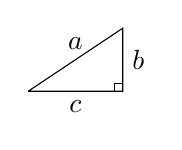
\begin{tikzpicture}[scale=0.40]
    \coordinate [] (A) at (-1.5cm,-1.cm);
    \coordinate [] (C) at (1.5cm,-1.0cm);
    \coordinate [] (B) at (1.5cm,1.0cm);
    \draw (A) -- node[above] {$a$} (B) -- node[right] {$b$} (C) -- node[below] {$c$} (A);
    \draw (1.25cm,-1.0cm) rectangle (1.5cm,-0.75cm);
\end{tikzpicture}
}


\begin{document}


\begin{center}
     \Large{\textbf{Python Programming}}\\
     \small{Class: COSC 1800}\hfill\small{\textcopyright Maximilien Notz \the\year{}}
     \noindent\rule{20.2cm}{0.4pt}
\end{center}


\begin{multicols}{2}
\setcounter{secnumdepth}{0}

\subsection{General Reminder}
\begin{tabular}{>{\ttfamily}l l}
    r.randint(x,y)      & Generate a random integer between \textbf{x}\\
                            & and \textbf{y}(import random as r).\\
        input(msg)          & Prompt the user with \textbf{msg} and take the\\
                            & user input.\\
        type(var)           & Returns the type of var.\\
        type(n, b, d,)      & Dynamically create a class named \textbf{n}.\\
                            & This class inherits all classes in \textbf{b} (tuple).\\
                            & \textbf{d} is a dictionary containing attributes\\
                            & and member method.\\
        int(var)            & Convert \texttt{var} to a integer.\\
        float(var)          & Convert \texttt{var} to a float.\\
        str(var)            & Convert \texttt{var} to a string.\\
        len(var)            & Returns the length of a string or a list.\\
        pass                & Used to keep an indentation empty\\
                            & avoiding \texttt{IndentationError}.\\
        .copy()             & Creates a new object but nested objects\\
                            & still reference the original.\\
        .deepcopy()         & Creates a new object with completely new\\
                            & copies of all nested objects.\\
        del var             & Deletes \texttt{var} from memory.\\
    \end{tabular}

\subsection{Operators}
\begin{tabular}{|>{\ttfamily}l|l|l|}
    \hline
    Symbol  &   Name                    & Type       \\
    \hline
    +       & addition                  & Arithmetic \\
    -       & subtraction               & Arithmetic \\
    *       & multiplication            & Arithmetic \\
    /       & division                  & Arithmetic \\
    \%      & modulo                    & Arithmetic \\
    **      & power                     & Arithmetic \\
    //      & div                       & Arithmetic \\
    and     & logical and               & Boolean    \\
    or      & logical or                & Boolean    \\
    not     & logical not               & Boolean    \\
    in      & \textbf{in}               & Membership \\
    ==      & equal                     & Comparison \\
    !=      & not equal                 & Comparison \\
    >       & greater than              & Comparison \\
    <       & less than                 & Comparison \\
    >=      & greater than or equal     & Comparison \\
    <=      & less than or equal        & Comparison \\
    \hline
\end{tabular}


\subsection{Error Handling}
\begin{minted}[bgcolor=LightGray]{Python}
try:   
    # risky operation
except ex:
    # runs if an exception of type ex is raised
else:
    # runs if no exception is raised
finally: 
    # Runs regardless of what happens
\end{minted}

\subsection{Data Structures}
\begin{tabular}{l>{\ttfamily}lll}
    list          & [e\_1, $\dots$]         & ordered, changeable, duplicates.\\
    tuple         & (e\_1, $\dots$)         & ordered, unchangeable, duplicates.\\
    set           & \{e\_1, $\dots$\}       & unordered, unchangeable,\\
                  &                         & no duplicates, unindexed.\\
    dictionary    & \{a\_1:b\_1, $\dots$\}  & ordered, changeable, no duplicates.\\
\end{tabular}

\subsubsection{Typing}
\texttt{import typing} to use type hints.\\
\begin{tabular}{>{\small\ttfamily}l l}
    Sequence      & ordered container supporting indexing and\\
                  & slicing.\\
    List          & mutable ordered sequence, supports indexing\\
                  & and append.\\
    Tuple         & immutable ordered sequence, fixed-size.\\
    Set           & unordered collection of unique elements.\\
    Dict          & mapping of keys to values.\\
    Mapping       & abstract read-only mapping interface.\\
    MutableMapping& mapping that supports mutation.\\
    Iterable      & can be iterated with for-loops.\\
    Iterator      & yields items on demand.\\
    Sized         & supports len().\\
    Hashable      & can be used as dict key or set element.\\
    Optional[T]   & either T or None.\\
    Union[A,B]    & value may be of type A or B.\\
    Any           & accepts any type.\\
\end{tabular}

\subsubsection{sets Methods}
\begin{tabular}{>{\ttfamily}l l}
    .add(e)                     & Add \texttt{e} in the set.\\
    .update(lst)                & Add all elements from \texttt{lst} in the set.\\
    .remove(e)                  & Remove \texttt{e} in the set.\\
    .union(lst)                 & add all elements from \texttt{lst}\\
    .intersection(lst)          & keep only the elements that are both in itself and \texttt{lst}\\
    .difference(lst)            & remove all element of \texttt{lst} in the set\\
\end{tabular}
\begin{tabular}{>{\ttfamily}l l}
    .symmetric\_difference(lst) & \\
\end{tabular}


\subsubsection{lists Methods}
\begin{minted}[bgcolor=LightGray]{Python}
    lst1 = [e_1, e_2, e_3] # [e_1, e_2, e_3]
    lst2 = 5 * [a] # [a, a, a, a, a]
    lst3 = [a for i in range(3)] # [a, a, a]
\end{minted}
\begin{tabular}{>{\ttfamily}l l}
    list(var)       & Convert a set or tuple to a list.\\
    lst[i]          & Access the \texttt{i}th element in the list.\\
    .append(a)      & Adds \texttt{a} to the end of the list.\\
    .insert(i,e)    & Insert element \texttt{e} at index \texttt{i}.\\
    .pop()          & Remove the last element, return the \\
                    & removed value.\\
    .pop(i)         & Remove element at index \texttt{i}, return the \\
                    & removed value.\\
    range(n)        & Create a list with all integers from \texttt{0} to \texttt{n}.\\
\end{tabular}

\subsubsection{dictionary Methods}
\begin{minted}[bgcolor=LightGray]{Python}
    dic = {"max":22, "ugo":40, "cyp":21}
    dic["max"] # -> 22
\end{minted}
\begin{tabular}{>{\ttfamily}l l}
 
\end{tabular}

\subsection{Regular Expressions(REGEX)}
\subsubsection{Functions}
Let \texttt{e} be a regular expression and \texttt{s} and \texttt{s2} be strings.
\begin{tabular}{>{\small\ttfamily}l l}
    import re               & include python REGEX library.\\
    .findall(e, s)          & Returns a list containing all matches of \texttt{e} in \texttt{s}.\\
    .search(e, s)           & Returns a Match object if there is a match of\\
                            & \texttt{e}  anywhere in \texttt{s}.\\
    .split(e, s)            & Returns a list where \texttt{s} has been split at each\\
                            & match of \texttt{e}.\\
    .sub(e, s2, s)          & Replaces one or many matches of \texttt{e} with \texttt{s2} in\\
                            & \texttt{s}, \small{optional parameter: number of replacements.}\\
    Match Object            & A Match Object is an object containing\\
                            & information about the search and the result.\\
                            & \small{Can act as a boolean that is true if not empty.}\\
\end{tabular}
\subsubsection{REGEX Syntax}


\textbf{Metacharacters:}\\
\begin{tabular}{>{\small\ttfamily}l l|>{\small\ttfamily}l l}
    \hline
    []                  & A set of chars                    & *     & Zero or more occurrences\\
    $\backslash$        & special sequence and              & +     & One or more occurrences\\
                        & escape special char               & ?     & Zero or one occurrences\\
    .                   & Any character except \texttt{$\backslash$n}  & {}    & Specify number of\\
    \textasciicircum    & Starts with                      &       & occurrences\\
    \$                  & Ends with                        & ()    & Capture and group\\
    |                   & Either or\\
    \hline
\end{tabular}

\textbf{Set Syntax by example:}\\
\begin{itemize*}
    \item \texttt{[aBc]} matches a single character: a, B, or c.
    \item \texttt{[\textasciicircum aBc]} matches any single character except a, B, or c.
    \item \texttt{[a-z]} matches any lowercase letter a through z.
    \item \texttt{[a-zA-Z]} matches any letter (uppercase or lowercase).
    \item \texttt{[0-9][0-9]} matches two consecutive digits (00-99).
\end{itemize*}

\textbf{Special Sequences:}\\
\begin{tabular}{>{\small\ttfamily}l l|>{\small\ttfamily}l l}
    \hline
    \textbackslash A & Match at start of string & \textbackslash d & Any digit [0-9]\\
    \textbackslash b & Word boundary            & \textbackslash D & Any non-digit\\
    \textbackslash B & Not a word boundary      & \textbackslash s & Any whitespace\\
    \textbackslash Z & Match at end of string   & \textbackslash S & Any non-whitespace\\
    \textbackslash w & Any word character       & \textbackslash W & Any non-word character\\
    \hline
\end{tabular}

\subsubsection{REGEX Backreferences}
Refer to earlier capturing groups in the pattern or in replacements. Prefer raw strings (e.g., \texttt{r"..."}) to avoid double escaping.
\begin{tabular}{>{\small\ttfamily}l l}
\textbackslash 1, \textbackslash 2, ...                 & Backreference to the nth capturing group in the\\
                                                        & pattern.\\
(?P<name>...)                                           & Named capturing group.\\
(?P=name)                                               & Backreference to the named group in the pattern.\\
\texttt{\textbackslash 1}, \texttt{\textbackslash 2}    & In replacement: refer to groups 1, 2 (works in\\
                                                        & \texttt{re.sub}).\\
\texttt{\textbackslash g<name>}                         & In replacement: recommended form for\\
                                                        & numeric/named groups.\\
\end{tabular}

\subsection{File Handling}
\begin{tabular}{>{\small\ttfamily}l l}
    open(s, arg)    & returns a a file object from a file at path \texttt{s}.\\
                    & file object can be iterated line by line.\\
    .read()         & returns a string version of a file.\\
    .read(n)        & returns a string version of a \texttt{n} first characters\\
                    & in file.\\
    .readline()     & returns return the next line of the file as a\\
                    & string.\\
    .close()        & Manually close a file.\\
    .write(s)       & writes string \texttt{s} to the file.\\
    .writelines(s)  & writes a list of strings \texttt{s} to the file.\\
\end{tabular}

\textbf{arguments for open():}
\begin{itemize*}
    \item \textbf{r:} read only (default).
    \item \textbf{w:} write only, creates or overwrites a file.
    \item \textbf{a:} append only, creates file if not existing.
    \item \textbf{b:} binary mode.
    \item \textbf{t:} text mode (default).
    \item \textbf{x:} create, fails if file exists.
    \item \textbf{+:} read and write.
\end{itemize*}

\subsubsection{with statement}
The \texttt{with} statement manages resources  resource management by automatically handling setup and cleanup tasks. 
For file handling, it ensures that files are properly closed when the block exits, even if an exception occurs.
\begin{minted}[bgcolor=LightGray]{Python}
with open("myFile.txt") as f:
  myString = f.read()
\end{minted}

\subsection{Object Oriented Programming(OOP)}
\begin{minted}[bgcolor=LightGray]{Python}
class ClassName(parent1, parent2, ...):
    var = value # class attribute with default value
    def __init__(self, arg1, ...): # constructor
        self.attr1 = arg1
        ...
    def method1(self, ...):
        # code
\end{minted}
\begin{tabular}{>{\small\ttfamily}l l}
    self        & reference to the current instance of the class.\\
    \_\_init\_\_  & constructor method called when an object is created.\\
    \_\_del\_\_ & destructor method called when an object is deleted.\\
\end{tabular}
\subsubsection{Operator Overloading}
\begin{tabular}{>{\small\ttfamily}l l}
    \_\_str\_\_(self)           & Overload \texttt{str()}.\\
    \_\_repr\_\_(self)          & Overload \texttt{repr()} (used by\\
                                & \texttt{print()}).\\
    \_\_add\_\_(self, o)        & + addition\\
    \_\_sub\_\_(self, o)        & - subtraction\\
    \_\_mul\_\_(self, o)        & * multiplication\\
    \_\_truediv\_\_(self, o)    & / division\\
    \_\_floordiv\_\_(self, o)   & // floor division\\
    \_\_mod\_\_(self, o)        & \% modulo\\
    \_\_pow\_\_(self, o)        & ** power\\
    \_\_neg\_\_(self)           & unary -\\
    \_\_pos\_\_(self)           & unary +\\
    \_\_abs\_\_(self)           & abs()\\
    \_\_eq\_\_(self, o)         & == equality\\ 
    \_\_ne\_\_(self, o)         & != inequality\\
    \_\_lt\_\_(self, o)         & $<$ less than\\
    \_\_le\_\_(self, o)         & $<=$ less or equal\\
    \_\_gt\_\_(self, o)         & $>$ greater than\\
    \_\_ge\_\_(self, o)         & $>=$ greater or equal\\
\end{tabular}

\subsection{Strings}
\begin{tabular}{>{\small\ttfamily}l l}
    str(var)        & Convert \texttt{var} to a string.\\
    .lower()        & Returns the string in lowercase.\\
    .upper()        & Returns the string in uppercase.\\
    .strip()        & Removes whitespace from the beginning\\
                    & and end of the string.\\
    .join(lst)      & Joins all elements in \texttt{lst} into a single\\
                    & string, separated by the original string.\\
    r"..."          & Raw string, ignores escape sequences.\\
    f"...\{var\}..."& Formatted string literal, inserts \texttt{var} inside the\\
                    & string.\\
    s[i:j]         & Slicing, returns substring from index \texttt{i}\\
                    & to \texttt{j-1}.\\
\end{tabular}

\subsection{Basic Syntax}
\begin{minted}[bgcolor=LightGray]{Python}
if condition_1:
    # code if condition_1 is true
elif condition_2:
    # code if condition_2 is true and condition_1 
    # is false
else:
    # code

def function(a:type1, b:type2 = value, ...) -> rType:
    # code
    return # value of type rType

for i in lst:
    # for each element in lst

while condition:
    # runs while condition is true
\end{minted}

\subsection{Performance Tips}


\end{multicols}
\end{document}
